\begin{figure}[H]
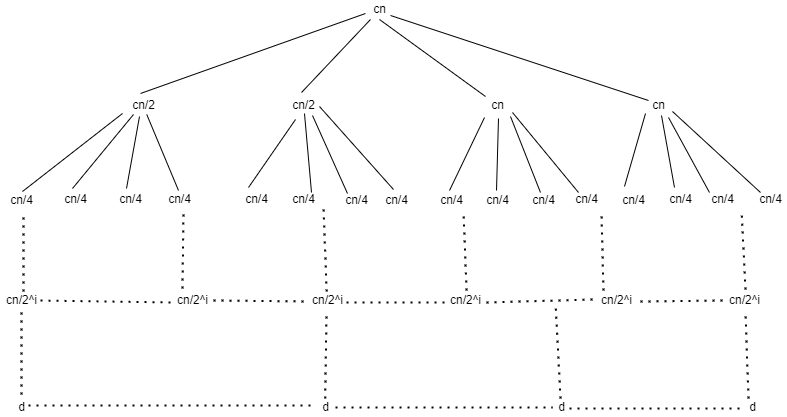
\includegraphics[scale=0.5]{Tree.png}
\end{figure}
\begin{tabular}{ccc}
Level &\#nodes &cost\\
0& 1 & cn \\
1 & 4 & $4\frac{cn}{2}$ \\
2 & 16 & $16\frac{cn}{4}$\\ 
.. & .. & ..\\
i & $2^{2i}$ & $2^{2i}\frac{cn}{2^i}$\\
.. & .. & ..\\
logn & $n^2$ & $n^2d$
\end{tabular}
Substitution method
\begin{equation*}
	\sum_{i = 0}^{logn - 1}2^icn + n^2d = cn\frac{2^0 - 2^{logn}}{1 - 2} + n^2d
\end{equation*} 
\begin{equation*}
	= - cn + cn^2 + n^2d = n^2(c + d - \frac{c}{n}) = \Theta(n^2)
\end{equation*} 
Master theorem
\begin{equation*}
	T(n) = 4T(\frac{n}{2}) + cn, T(1) = d
\end{equation*}
$a = 4$, $b = 2$, $f(n) = cn$
\begin{equation*}
	n^{logba} = n^{log_24} = n^2
\end{equation*} 
We have $f(n) = O(n^{2 - \epsilon})$, with $\epsilon = 0.5$. For case 1 of the master theorem:
\begin{equation*}
	T(n) = \Theta(n^2)
\end{equation*}